\chapter{Theory}
\section{Furuta's Pendulum}
\subsection{Device Overview}
Rotational inverted pendulum or Furuta’s pendulum was firstly invented in 1992 at the Tokyo Institute of Technology by Katsuhisa Furuta as an example of a complex nonlinear oscillator in the sake of control algorithms testing in process control theory.
The pendulum composes of motor-driven arm, which rotates in the horizontal plane and a pendulum, attached to that arm, which freely rotates in the vertical plane. The system is underactuated and extremely nonlinear due to the gravitational forces and the coupling arising from the Coriolis and centripetal forces. The schematic representation of the pendulum is shown in \ref{furuta}
\begin{figure}[h]
	\centering
	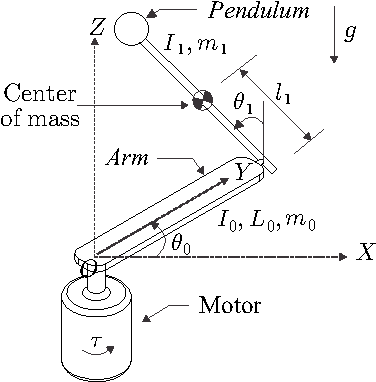
\includegraphics[width=.55\linewidth]{images/furuta}
	\caption{Furuta's Pendulum}
	\label{furuta}
\end{figure}
\newpage
Consider the rotational inverted pendulum
mounted to a DC motor as shown in (\ref{furuta}). The DC motor
is used to apply a torque $\tau$ to Arm. The link between Arm and Pendulum is not actuated but free to rotate. The two arms have lengths $L_0$ and $L_1$. The arm and pendulum have masses $m_1$ and $m_2$ which are located at $l_0$ and $l_1$, respectively, which are the lengths from the point of rotation of the arm to its center of mass. The arm and the pendulum have inertia tensors $J_0$ and $J_1$ (about the centre of mass of the arm).
A right hand coordinate system has been used to define the inputs, states, and the Cartesian coordinate systems 0 and 1. The coordinate axes of Arm and Pendulum are the principalaxes, such that the inertia tensors are diagonal of the form
\begin{subequations}
	\begin{align}
		J_0 = 	\begin{bmatrix}
					J_{0xx} & 0 & 0\\
					0 & J_{0yy} & 0\\
					0 & 0 & J_{0zz}\\
				\end{bmatrix},\\
		J_1 = 	\begin{bmatrix}
					J_{1xx} & 0 & 0\\
					0 & J_{1yy} & 0\\
					0 & 0 & J_{1zz}\\
				\end{bmatrix}.
	\end{align}
\end{subequations}
\begin{table}[h]
	\caption{Parametres of Furuta pendulum}
	\begin{tabular}
		{l l l}
		\noalign{\hrule height 1pt}
		Symbol&Parameter&Unit\\
		\noalign{\hrule height 1pt}
		$g$&gravitational acceleration&\si{\metre\per\square\second}\\
		$m_0$&mass of arm&\si{\kilogram}\\
		$m_1$&mass of pendulum&\si{\kilogram}\\
		$L_0$&length of arm&\si{\metre}\\
		$L_1$&length of pendulum&\si{\metre}\\
		$l_0$&location of the arms center of mass&\si{\metre}\\
		$l_1$&location of the pendulums center of mass&\si{\metre}\\
		$I_0$&moment of inertia of arm&\si{\kilogram\per\square\metre}\\
		$I_1$&moment of inertia of pendulum&\si{\kilogram\per\square\metre}\\
		$\theta_0$&arm angle&\si{\radian}\\
		$\theta_1$&pendulum angle&\si{\radian}\\
		$\tau$&motor torque&\si{\volt}\\
		\hline
	\end{tabular}
\end{table}
\subsection{Lagrangian Formulation}
To design a predictive controller, the knowledge of the dynamic model of the process is necessary. The analytical model based on the equations of motion could be derived from the Lagrange equations \cite{furuta:model}, which represent the most commonly used method for establishing equations of motion of difficult mechanical systems.
\subsubsection{Rotation Matrices}
First, define two rotation matrices
which are used in both the Lagrange formulation. The rotation matrix from the base to Arm is
\begin{equation}
	R_0 = 	\begin{bmatrix}
					\ \ \,\cos(\theta_0) & \sin(\theta_0) & 0\\
					-\sin(\theta_0) & \cos(\theta_0) & 0\\
					0 & 0 & 1
				\end{bmatrix}.
\end{equation}
The rotation matrix from Arm to Pendulum is derived by
initially applying a (diagonal) matrix to that maps the frame
0 to frame 1, followed by a rotation matrix for $\theta_1$, given by
\begin{equation}
R_1 = 	\begin{bmatrix}
			0 & \sin(\theta_1) & -\cos(\theta_1)\\
			0 & \cos(\theta_1) & \ \ \,\sin(\theta_1)\\
			1 & 0 & 0                      
		\end{bmatrix}.
\end{equation}
\subsubsection{Velocities}
The angular velocity of Arm is given by
\begin{equation}
	\omega_0 = 	\begin{bmatrix}
					0 & 0 & \dot{\theta}_0
				\end{bmatrix}^\intercal.
\end{equation}
Let the velocity of the base frame be at rest, such that the joint
between the frame and the Arm is also at rest, that is,
\begin{equation}
	\text{\textbf{v}}_0 = 	\begin{bmatrix}
					0 & 0 & 0
			\end{bmatrix}^\intercal.
\end{equation}
The total linear velocity of the centre of mass of Arm is
given by
\begin{equation}
	\text{\textbf{v}}_{0c} = v_0+\omega_0\times\begin{bmatrix}
					l_0 & 0 & 0
				\end{bmatrix}^\intercal = \begin{bmatrix}
				0 & \dot{\theta}_0l_0 & 0
				\end{bmatrix}^\intercal.
\end{equation}
The angular velocity of the Pendulum is given by
\begin{equation}
\omega_1 = R_1\omega_0 + \begin{bmatrix}
				0 & 0 & \dot{\theta}_1
			\end{bmatrix}^\intercal = 
			\begin{bmatrix}
				-\cos(\theta_1)\dot{\theta}_0 & \sin(\theta_1)\dot{\theta}_0 & \dot{\theta}_1
			\end{bmatrix}^\intercal.
\end{equation}
The velocity of the joint between Arm and the pendulum in
reference frame 1 is
\begin{equation}
	\text{\textbf{v}}_{1} = R_1\lrp{\omega_0\times	\begin{bmatrix}
									L_0 & 0 & 0
									\end{bmatrix}^\intercal} = 
	\begin{bmatrix}
		\dot{\theta}_0L_0\sin(\theta_1)\\
		\dot{\theta}_0L_0\cos(\theta_1)\\
		0
	\end{bmatrix}.
\end{equation}
The total linear velocity of the centre of mass of Arm 2 is
given by
\begin{equation}
	\text{\textbf{v}}_{1c} = \text{\textbf{v}}_1+\omega_1\times\begin{bmatrix}
																	l_1 & 0& 0
															\end{bmatrix}^\intercal=
	\begin{bmatrix}
		\dot{\theta}_0L_0\sin(\theta_1)\\
		\dot{\theta}_0L_0\cos(\theta_1) + \dot{\theta}_1l_1\\
		-\dot{\theta}_0l_1\sin(\theta_1)
	\end{bmatrix}.														
\end{equation}
\subsubsection{Energies}
The potential energy of Arm is
\begin{equation}
	\ui{E}{p0} = 0,
\end{equation}
and the kinetic energy is
\begin{equation}
	\ui{E}{k0} = \frac{1}{2}\lrp{\text{\textbf{v}}_{0c}^\intercal m_0\textbf{v}_{0c} + \omega_0^\intercal J_0\omega_0 } = 
	\frac{1}{2}\dot{\theta}_0^2\lrp{ m_0l_0^2+J_{0zz} }.
\end{equation}
The potential energy of the Pendulum is
\begin{equation}
\ui{E}{p1} = gm_1l_1\lrp{1-\cos(\theta_1)},
\end{equation}
and the kinetic energy is
\begin{equation}
\begin{split}
	\ui{E}{k1} = &\frac{1}{2}\lrp{\text{\textbf{v}}_{1c}^\intercal m_1\textbf{v}_{1c} + \omega_1^\intercal J_1\omega_1 }\\
	= &\frac{1}{2}\dot{\theta}_0^2\lrp{m_1L_1^2+\lrp{m_1l_1^2+J_{1yy}}\sin^2(\theta_1)+J_{1xx}\cos^2(\theta_1)}\\
	&+\frac{1}{2}\dot{\theta}_1^2\lrp{ J_{1zz}+m_1l_1^2 }+m_1L_0l_1\cos(\theta_1)\dot{\theta}_0\dot{\theta}_1.
\end{split}
\end{equation}
The total potential and kinetic energies are given, respectively, by
\begin{subequations}
	\begin{align}
		\ui{E}{p} &= \ui{E}{p0} + \ui{E}{p1}, \\
		\ui{E}{k} &= \ui{E}{k0} + \ui{E}{k1}.
	\end{align}
\end{subequations}
\subsubsection{Lagrangian}
The Lagrangian is the difference in kinetic and potential energies
\begin{equation}
	L = \ui{E}{k} - \ui{E}{p}.
\end{equation}
From this, we obtain the Euler-Lagrange equations for two degrees of freedom system
\begin{subequations}
	\begin{align}
		\dif{}{t}\lrp{\diff{L}{\dot{\theta}_0}}-\diff{L}{\dot{\theta}_0} = \tau,\\
		\dif{}{t}\lrp{\diff{L}{\dot{\theta}_1}}-\diff{L}{\dot{\theta}_1} = 0.
	\end{align}
\end{subequations}
Evaluating the terms of those Euler-Lagrange equations and following substitution gives the following equations of motion
\begin{subequations}
	\begin{align}
	\ddot{\theta}_0 &= \frac{\gamma(\epsilon\dot{\theta}_0^2+\rho)-\delta(\tau+\beta\dot{\theta}_1^2-\sigma\dot{\theta}_0\dot{\theta}_1)}{\gamma^2-\alpha\delta}\label{motion1},\\
	\ddot{\theta}_1 &= \frac{\gamma(\tau+\beta\dot{\theta}_1^2-\sigma\dot{\theta}_0\dot{\theta}_1)-\alpha(\epsilon\dot{\theta}_0^2+\rho)}{\gamma^2-\alpha\delta}\label{motion2},
	\end{align}
\end{subequations}
where
\begin{subequations}
	\begin{align}
	\alpha &= I_0+L_0^2m_1+l_1^2m_1\sin^2\theta_1,\\
	\beta &= L_0m_1l_1\sin\theta_1, \\
	\gamma &= L_0m_1l_1\cos\theta_1,\\
	\delta &= I_1+l_1^2m_1,\\
	\epsilon &= l^2_1m_1\sin\theta_1\cos\theta_1,\\
	\rho &= m_1gl_1\sin\theta_1,\\
	\tau &= 2l^2_1m_1\sin\theta_1\cos\theta_1.
	\end{align}
\end{subequations}
\subsection{State-Space Reprentation} 
To obtain the state representation of the process the state variables must be defined first:
\begin{equation}
\begin{bmatrix}
x_1(t)&x_2(t)&x_3(t)&x_4(t)
\end{bmatrix}^\intercal = 
\begin{bmatrix}
\theta_0(t)&\dot{\theta}_0(t)&\theta_1(t)&\dot{\theta}_1(t)
\end{bmatrix}^\intercal.
\end{equation}
And the control variable:
\begin{equation} u(t) = \tau(t). \end{equation}
\subsubsection{Nonlinear Model}
Equations (\ref{motion1}) and (\ref{motion2}) are further utilized to establish the state
space model
\begin{subequations}
	\begin{align}
	\dot{x}_1 &= \dot{\theta_0}, \\
	\dot{x}_2 &= \frac{\gamma(\epsilon\dot{\theta_0}^2+\rho)-\delta(\tau+\beta\dot{\theta_1}^2-\sigma\dot{\theta_0}\dot{\theta_1})}{\gamma^2-\alpha\delta},\\
	\dot{x}_3 &= \dot{\theta_1},\\
	\dot{x}_4 &= \frac{\gamma(\tau+\beta\dot{\theta_1}^2-\sigma\dot{\theta_0}\dot{\theta_1})-\alpha(\epsilon\dot{\theta_0}^2+\rho)}{\gamma^2-\alpha\delta}.
	\end{align}
\end{subequations}
Now these non-linear differential equations could be written in the form of matrices:
\begin{equation}\label{nonlinmodel}
\begin{bmatrix}
\dot{x}_1(t) \\ \dot{x}_2(t) \\ \dot{x}_3(t) \\ \dot{x}_4(t)
\end{bmatrix} = \begin{bmatrix}
\dot{\theta}_0\\
\frac{\gamma(\epsilon\dot{\theta}_0^2+\rho)-\delta(\tau+\beta\dot{\theta}_1^2-\sigma\dot{\theta}_0\dot{\theta}_1)}{\gamma^2-\alpha\delta}\\
\dot{\theta}_1\\
\frac{\gamma(\tau+\beta\dot{\theta}_1^2-\sigma\dot{\theta}_0\dot{\theta}_1)-\alpha(\epsilon\dot{\theta}_0^2+\rho)}{\gamma^2-\alpha\delta}
\end{bmatrix}.
\end{equation}
As we can see the derivatives of the states are the functions of the current states and control input. And more importantly, those variables have nonlinear interactions within each dynamic equation. 
\begin{equation}\begin{bmatrix}
\dot{x}_1(t) \\ \dot{x}_2(t) \\ \dot{x}_3(t) \\ \dot{x}_4(t)
\end{bmatrix} = f(x(t),u(t)) =\begin{bmatrix}f_1(x(t),u(t))\\f_2(x(t),u(t))\\f_3(x(t),u(t))\\f_4(x(t),u(t))\end{bmatrix}. \end{equation}
\subsubsection{Linear Model}
Non-linear model (\ref{nonlinmodel}) can be approximated around operation point by a linear, time-invariant state-space model in the following form
\begin{equation}\dot{x}(t) = Ax(t) + Bu(t).\end{equation}
Its constant matrices can be obtained by calculating its partial derivatives with respect to the state and control variables.
\begin{subequations}
	\begin{align}
	A &= \begin{bmatrix}
	\frac{\partial f_1(x(t),u(t))}{\partial x_1}&\frac{\partial f_1(x(t),u(t))}{\partial x_2}&\frac{\partial f_1(x(t),u(t))}{\partial x_3}&\frac{\partial f_1(x(t),u(t))}{\partial x_4}\\
	\frac{\partial f_2(x(t),u(t))}{\partial x_1}&\frac{\partial f_2(x(t),u(t))}{\partial x_2}&\frac{\partial f_2(x(t),u(t))}{\partial x_3}&\frac{\partial f_2(x(t),u(t))}{\partial x_4}\\
	\frac{\partial f_3(x(t),u(t))}{\partial x_1}&\frac{\partial f_3(x(t),u(t))}{\partial x_2}&\frac{\partial f_3(x(t),u(t))}{\partial x_3}&\frac{\partial f_3(x(t),u(t))}{\partial x_4}\\
	\frac{\partial f_4(x(t),u(t))}{\partial x_1}&\frac{\partial f_4(x(t),u(t))}{\partial x_2}&\frac{\partial f_4(x(t),u(t))}{\partial x_3}&\frac{\partial f_4(x(t),u(t))}{\partial x_4}
	\end{bmatrix},\\ 
	B &= \begin{bmatrix}
	\frac{\partial f_1(x(t),u(t))}{\partial u}\\\frac{\partial f_2(x(t),u(t))}{\partial u}\\\frac{\partial f_3(x(t),u(t))}{\partial u}\\\frac{\partial f_4(x(t),u(t))}{\partial u}
	\end{bmatrix}.
	\end{align}
\end{subequations}
And when we compute these derivatives, we obtain a linearized continuous-time dynamic model of the pendulum in the form of state matrices
\begin{subequations}\label{linmatrices}
	\begin{align}
	A &=\begin{bmatrix}0&1&0&0\\
	0&0&\frac{-gL_0l_1^2m_1^2}{(m_1L_0^2+I_0)(m_1l_1^2+I_1)-L_0^2l_1^2m_1^2}&0\\
	0&0&0&1\\
	0&0&\frac{gl_1m_1(m_1L_0^2+I_0)}{(m_1L_0^2+I_0)(m_1l_1^2+I_1)-L_0^2l_1^2m_1^2}&0
	\end{bmatrix},\\
	B &=	\begin{bmatrix}
	0\\ 
	\frac{m_1L_1^2+I_1}{(m_1L_0^2+I_0)(m_1l_1^2+I_1)-L_0^2l_1^2m_1^2}\\
	0\\
	\frac{-L_0l_1m_1}{(m_1L_0^2+I_0)(m_1l_1^2+I_1)-L_0^2l_1^2m_1^2}
	\end{bmatrix},\\
	C &= \begin{bmatrix}0&0&1&0\end{bmatrix},\\
	D &= 0.
	\end{align}
\end{subequations}
Now those linearized equations of motion would be evaluated at two equilibrium positions: upright and downward. The reason is that at the downward position the system's output, which is the position of the pendulum, has a stable point at “$+\pi$” and “$-\pi$”, while at the upright position system has no stable point.

The model, obtained by linearization around the upright operation point, is used for fulfilling the main control objective, which is stabilizing the pendulum at the upright position. The second model is used to simulate process behavior during initial excitation by a Swing-up controller.
\section{Controller Theory}
In this section theory for the individual controllers is described. As we are aiming for swing-up control of the pendulum, several controllers should be designed. For the heuristic swing-up approach an energy shaping controller and a predictive controller. And for the optimal swing-up approach a nonlinear model predictive control strategy.
\subsection{Model Predictive Control}\label{mpcsection}
Model Predictive Control (MPC) uses a model of the system to make predictions about the system’s future behavior. MPC solves an online optimization algorithm to find the optimal control action that drives the predicted output to the reference. MPC can handle MIMO systems that may have interactions between their inputs and outputs. It can also handle input and output constraints. MPC has preview capability; it can incorporate future reference information into the control problem to improve controller performance. Due to all these properties MPC provides the highest quality of control performance at the moment.
\subsubsection{Model Predictive Control Formulation}
The model predictive control requires the linear discrete-time state-space model of the process
\begin{subequations}\label{linmodel}
	\begin{align}	
	x_{k+1} = Ax_k + Bu_k,\\
	y_k = Cx_k + Du_k.
	\end{align}
\end{subequations}
Thanks to the knowledge of that model, we can predict the evolution of states and outputs of the system.\\
Due to the setup of the controlled process, the MPC should be formulated to regulate the states of the system to the origin. And such MPC can be formulated as
\begin{subequations}\label{mpcgeneral}
	\begin{align}
		\min_{U}\ \sum_{k=0}^{N-1}& \lrp{\left\| \ui{Q}{x}x_{k}\right\|_2+\left\|\ui{Q}{u}u_{k}\right\|_2}\\
	    \label{eq217b}\text{s.t.}\qquad&x_{k+1} = Ax_{k} + Bu_{k}\qquad\quad  k \in \mathbb{N}_0^{N-1}\\
		&x_0 = x(0)\\
		\label{cst_x}&x_{k}\in\mathcal{X}\qquad\qquad\qquad\qquad\,  k \in \mathbb{N}_0^{N-1}\\
		\label{cst_u}&u_{k}\in\mathcal{U}\qquad\qquad\qquad\qquad\;   k \in \mathbb{N}_0^{N-1}
	\end{align}
\end{subequations}
where $\mathcal{X}$ and $\mathcal{U}$ are polytopic state and input constraints respectively and defined as
\begin{subequations}
	\begin{align}
	\mathcal{X} &= \{\ui{H}{x}x_k\leq \ui{K}{x}\},\\
	\mathcal{U} &= \{\ui{H}{u}u_k\leq \ui{K}{u}\}.
	\end{align}
\end{subequations}
In case of box constraints
\begin{subequations}
	\begin{align}
		\ui{x}{min}\leq x_k \leq\ui{x}{max},\\
		\ui{u}{min}\leq x_k \leq\ui{u}{max},\\
	\end{align}
\end{subequations}
the matrices $\ui{H}{x}$, $\ui{K}{x}$, $\ui{H}{u}$ and $\ui{K}{u}$ have the following form
\begin{subequations}
	\begin{align}
		\ui{H}{x} = \begin{bmatrix}
						\ \ \,I\\-I
					\end{bmatrix},\quad & 
		\ui{K}{x} = \begin{bmatrix}
						\ \ \,\ui{x}{max}\\-\ui{x}{min}
					\end{bmatrix},\\
		\ui{H}{u} = \begin{bmatrix}
						\ \ \,I\\-I
					\end{bmatrix},\quad & 
		\ui{K}{u} = \begin{bmatrix}
						\ \ \,\ui{u}{max}\\-\ui{u}{min}
					\end{bmatrix}.
	\end{align}
\end{subequations}
Unfortunately, such formulation is inappropriate for quadratic programming solver, so it has to be reformulated in the form of a quadratic optimization problem.
\subsubsection{Model Predictive Control as a Quadraic Programming Optimization Problem}
To solve an MPC problem, the Quadratic Programming (QP) solver is used. Unfortunately, an MPC formulation (\ref{mpcgeneral}) is inappropriate for QP solver and has to be reformulated. The standard QP problem has the following form
\begin{subequations}
	\begin{align}
	\min_{z}\quad & z^\intercal Pz + 2Q^\intercal z + R\\
	\label{cst_qp}\text{s.t.}\quad&Hz\leq G\\
	&\ui{H}{eq}z = \ui{G}{eq}
	\end{align}
\end{subequations}
As the first step, the standard MPC cost function should be written in a vector form
\begin{equation}
	\min_{U}\quad X^\intercal\ui{\tilde{Q}}{x}X + U^\intercal\ui{\tilde{Q}}{u}\,U\\
\end{equation}
where $X$ is a vector of predicted states, $U$ is an optimal trajectory of future control inputs and $\ui{\tilde{Q}}{x}$ and $\ui{\tilde{Q}}{u}$ are the matrices of original weight matrices.
\begin{equation}
	X = \begin{bmatrix}
	x_0\\x_{1}\\\vdots\\x_{N-1}
		\end{bmatrix},
\end{equation}
\begin{equation}
U = \begin{bmatrix}
u_0\\u_{1}\\\vdots\\u_{N-1}
\end{bmatrix},
\end{equation}
\begin{equation}
\ui{\tilde{Q}}{x} = \begin{bmatrix}
\ui{Q}{x}&0&\cdots&0\\
0&\ui{Q}{x}&\cdots&0\\
\vdots&\vdots&\ddots&\vdots\\
0&0&\cdots&\ui{Q}{x}
\end{bmatrix},
\end{equation}
\begin{equation}
\ui{\tilde{Q}}{u} = \begin{bmatrix}
\ui{Q}{u}&0&\cdots&0\\
0&\ui{Q}{u}&\cdots&0\\
\vdots&\vdots&\ddots&\vdots\\
0&0&\cdots&\ui{Q}{u}
\end{bmatrix}.
\end{equation}
At the next step, the equality constrains (\ref{eq217b}) should be expressed in the vector form. We can achieve that by predicting the evolution of states over the whole prediction horizon.
\begin{equation}
\begin{split}
x_0 &= x(t)\\
x_{1} &= Ax_0 + Bu_0\\
x_{2} &= A\hat{x}_{1} + Bu_{1}\\
&= A^2x_0 + ABu_0 + Bu_{1}\\
x_{3} &= A\hat{x}_{2} + Bu_{2}\\
&= A^3x_0 + A^2Bu_0 + ABu_{1} + Bu_{2}\\
&\vdots\\
x_{k} &= A^kx_0+\sum_{j=0}^{k-1}A^jBu_{k-j-1}
\end{split}
\end{equation}
Or, if we write these equations in a compact form, we obtain
\begin{equation}
	\begin{bmatrix}
	x_0\\x_{1}\\ x_{2}\\\vdots\\ x_{N-1}
	\end{bmatrix} = 
	\begin{bmatrix}I\\A\\A^2\\ \vdots \\ A^{N-1}\end{bmatrix}x_0 + 
	\begin{bmatrix}
	0& 0&\cdots&0&0\\
	B&0&\cdots&0&0\\
	AB&B&\cdots&0&0\\
	\vdots&\vdots&\ddots&\vdots&\vdots\\
	A^{N-2}B&A^{N-3}B&\cdots&B&0\end{bmatrix}
	\begin{bmatrix}u_0\\u_{1}\\u_{2}\\\vdots\\u_{N-1}\end{bmatrix}.
\end{equation}
Or in the short form
\begin{equation}\label{eq227}
	X = \tilde{A}x_0 + \tilde{B}U.
\end{equation}
At this point, we can substitute as $X$ in the cost function by (\ref{eq227}). Then we obtain the new objective function
\begin{equation}\label{eq228}
	\min_{U}\ (\tilde{A}x_0 + \tilde{B}U)^\intercal\ui{\tilde{Q}}{x}(\tilde{A}x_0 + \tilde{B}U) + U^\intercal\ui{\tilde{Q}}{u}\,U.
\end{equation}
And when we expand and simplfie (\ref{eq228}), we obtain
\begin{equation}
	U^\intercal(\tilde{B}^\intercal\ui{\tilde{Q}}{x}\tilde{B} + \ui{\tilde{Q}}{u})U + 2x_0^\intercal\tilde{A}^\intercal\ui{\tilde{Q}}{x}\tilde{B}U + x_0^\intercal\tilde{A}\ui{\tilde{Q}}{x}\tilde{A}x_0.
\end{equation}
Now if we define $z = U$, we can cleary see matrices $P$, $Q$ and $R$, which occurs in a standart cost function for the quadratic optimization.
\begin{subequations}
	\begin{align}
		P &= \tilde{B}^\intercal\ui{\tilde{Q}}{x}\tilde{B} + \ui{\tilde{Q}}{u},\\
		Q &= (2x_0^\intercal\tilde{A}^\intercal\ui{\tilde{Q}}{x}\tilde{B}U)^\intercal,\\
		R &= x_0^\intercal\tilde{A}\ui{\tilde{Q}}{x}\tilde{A}x_0.
	\end{align}
\end{subequations}
Now only constrains remain. Constrains (\ref{cst_x}) and (\ref{cst_u}) must be reformulated as (\ref{cst_qp}). Those constrains we consider as a upper and lower bounds for the states and control inputs respectively
\begin{subequations}
	\begin{align}
		\ui{x}{min} &\leq x_k \leq \ui{x}{max} \quad k \in \mathbb{N}_0^{N-1}\\
		\ui{u}{min} &\leq u_k \leq \ui{u}{max} \quad k \in \mathbb{N}_0^{N-1}
	\end{align}
\end{subequations}
Now we split and vectorise those constrains
\begin{subequations}
\begin{align}
	X &\leq \ \; \, \ui{X}{max},\\
	-X &\leq -\ui{X}{min},\\
	U &\leq \ \; \, \ui{U}{max},\\
	-U &\leq -\ui{U}{min}.
\end{align}
\end{subequations}
In the next step, $X$ in the states constrains is substituted by a (\ref{eq227}) and $U$ expressed
\begin{subequations}
	\begin{align}
	\tilde{B}\,U &\leq \ \; \,\ui{X}{max} - \tilde{A}x_0,\\
	-\tilde{B}\,U &\leq -\ui{X}{min} + \tilde{A}x_0,\\
	U &\leq \ \; \,\ui{U}{max},\\
	-U &\leq -\ui{U}{min}.
	\end{align}
\end{subequations}
Those constraints are in the standard form and by combining them, we obtain matrices of inequality constraints $H$ and $G$ for the quadratic programming problem
\begin{equation}
	H = \begin{bmatrix}
	\ \; \,\tilde{B}\\
	-\tilde{B}\\
	\ \ \, I\\
	-I\\
	\end{bmatrix}, \quad
	G = \begin{bmatrix}
	\ \; \,\ui{X}{max} - \tilde{A}x_0\\
	-\ui{X}{min} + \tilde{A}x_0\\
	\ \ \:\ui{U}{max}\\
	-\ui{U}{min}
	\end{bmatrix}.
\end{equation}
At this point, as matrices $R$, $Q$, $R$, $H$ and $G$ are defined, and MPC strategy can be implemented via using any QP solver.
\subsection{Energy Shaping Controller}\label{energyshapingsection}
For the initial excitation of the system, we use the energy-based swing-up controller. The strategy with this controller is that we increase the amplitude of swings by increasing the energy of the system with every swing. The energy is added by controlling arms movements and depends on the actual energy of the pendulum. The actual energy of the pendulum can be calculated from the actual position of the pendulum and its velocity: 
\begin{equation}
E = \frac{m_1gl_1}{2}\lrp{\lrp{\frac{\dot{\theta}_1}{\omega_0}}^2+\cos\theta_1 - 1}.
\end{equation}
Than the control law has following form:
\begin{equation}\label{energy-shaping}
	u = \ui{k}{v}E\,\mathrm{sign}\lrp{\dot{\theta}_1\cos\theta_1}.
\end{equation}
Where element $\mathrm{sign}\lrp{\dot{\theta_1}\cos\theta_1}$ determines direction i which the force will be applied and $\ui{k}{v}$ is the gain of the controller.
\newpage
\subsection{Nonlinear Model Predictive Control}\label{nmpcsection}
To control the process, MPC uses a model of the process to predict the evolution of states and outputs of the process in the following sampling periods. In general, the process dynamics are complex and cannot be described perfectly. Any modeling method introduces some uncertainties into the resulting model. For example, the linear model is valid only in som range around the linearization point. So linear MPC, which uses such could be designed to control the process only in that range. But nonlinear modeling is a much more precise approach to describe the process dynamic. And in the case of Furuta pendulum, its full range dynamic can be described by a nonlinear model (\ref{nonlinmodel}). And by using such a model to predict the behavior of the process an NMPC strategy to perform Swing-Up control of the pendulum can be designed.

To design an optimal controller, an optimization problem has to be solved. In case of NMPC a Nonlinear Programing (NLP) problem is solved
\begin{subequations}\label{nlpgeneral}
	\begin{align}
	\min_{x}\  &f(x)\\
	\text{s.t.}\  &h(x) = 0\\
		 &g(x)\leq 0
	\end{align}
\end{subequations}
Sometimes, to obtain an analytical solution to such problem, could be extremely difficult. So a numerical method called Sequential Quatratic Programming (SQP) is used instead.
\subsubsection{Sequential Quatratic Programming}
Sequential Quadratic Programming is arguably become the most successful method for solving nonlinearly constrained optimization problems \cite{SQP:Theory}. Its general idea is to approximate NLP at current iterate by QP subproblem, solve that subproblem, than use the solution to construct a new iterate. This construction is done in such a way that the sequence converges to a local minimum of the NLP.

The main condition for a QP subproblem is that it has to reflect the properties of NLP at current iteration. But before such subproblem could be constructed, a few terms should be establish first.
\begin{itemize}
	\item Lagrangian functional of the NLP, $\mathcal{L}$ is defined as\begin{equation}
		\mathcal{L}(x,\lambda,\mu) = f(x) + \lambda^\intercal h(x) + \mu^\intercal g(x). 
	\end{equation}
	\item The gradient of $f$, $\nabla f(x)$ is denoted as
	\begin{equation}
		\nabla f(x) = \lrp{\diff{f(x)}{x_1},\diff{f(x)}{x_2},\cdots,\diff{f(x)}{x_n}}^\intercal.
	\end{equation}
	\item Hessian of f, $Hf(x)$ is the matrix of second partial derivatives as given by
	\begin{equation}
		\lrp{Hf(x)}_{ij} := \diffxy{f(x)}{x_i}{x_j}.
	\end{equation}
\end{itemize}
A major concern in SQP method is the choice of appropriate quadratic subproblem. 
The most obvious choice for the objective functional in this quadratic program is its local quadratic approximation
\begin{equation}
f(x)\approx f(x_k)+\nabla f(x_k)\lrp{x-x_k}+\frac{1}{2}\lrp{x-x_k}^\intercal Hf(x_k)\lrp{x-x_k}.
\end{equation}
and the constraint functions $h$ and $g$ by their local affine approximations
\begin{subequations}
	\begin{align}
		h(x)&\approx h(x_k)+\nabla h(x_k)\lrp{x-x_k},\\
		g(x)&\approx g(x_k)+\nabla g(x_k)\lrp{x-x_k}.	
	\end{align}
\end{subequations}
And after setting 
\begin{subequations}
	\begin{align}
		d_x&=x-x_k,\\
		B_k &= Hf(x_k).
	\end{align}
\end{subequations}
The following form of the QP subproblem is accured
\begin{subequations}
	\begin{align}
		\min_{d_x}\  &\nabla f(x_k)^\intercal d_x+\frac{1}{2}d_x^\intercal B_k d_x\\
		\text{s.t.}\  &h(x_k)+\nabla h(x_k)\lrp{x-x_k} = 0\\
		&g(x_k)+\nabla g(x_k)\lrp{x-x_k}\leq 0
	\end{align}
\end{subequations}
This is a reasonable approximation in case of linear constraints. In case of nonlinear constraints makes such choice inappropriated. 

To take nonlinearities in the constraints into account a quadratic model of the Lagrangian function could be used as the obective instead.
\begin{subequations}
	\begin{align}
	\min_{x}\  & \mathcal{L}(x,\lambda^*,\mu^*)\\
	\text{s.t.}\  &h(x)= 0\\
	&g(x)\leq 0
	\end{align}
\end{subequations}
Although the optimal multipliers are unknown, then approximations $\lambda_k$,$\mu_k$ could be contained as part of the iterative process. Then at a current iterate $(x_k,\lambda_k,\mu_k)$, the objective functional in stems from the quadratic Taylor series approximation.
\begin{equation}
	\mathcal{L}(x_k,\lambda_k,\mu_k)+\nabla\mathcal{L}(x_k,\lambda_k,\mu_k)^\intercal d(x)+\frac{1}{2}d(x)^\intercal H\mathcal{L}(x_k,\lambda_k,\mu_k) d(x).
\end{equation}
What leads to the final QP subproblem
\begin{subequations}
	\begin{align}
	\min_{d_x}\  &\nabla \mathcal{L}(x_k,\lambda_k,\mu_k)^\intercal d_x+\frac{1}{2}d_x^\intercal H\mathcal{L}(x_k,\lambda_k,\mu_k)d_x\\
	\text{s.t.}\  &h(x_k)+\nabla h(x_k)\lrp{x-x_k} = 0\\
	&g(x_k)+\nabla g(x_k)\lrp{x-x_k}\leq 0
	\end{align}
\end{subequations}
By solving that QP subproblem solution $d_x$ as well as local optimal values of multipliers $\lambda_{qp}$ and $\mu_{qp}$ are accuried, and setting 
\begin{subequations}
	\begin{align}
		d_\lambda &= \lambda_{qp}-\lambda_k,\\
		d_\mu &= \mu_{qp}-\mu_k.
	\end{align}
\end{subequations}
allow the updates of $(x,\lambda,\mu)$ to be written in the compact form
\begin{subequations}
	\begin{align}
	x_{k+1} &= x_k + \alpha d_x,\\
	\lambda_{k+1} &= \lambda_k + \alpha d_\lambda,\\
	\mu_{k+1} &= \mu_k + \alpha d_\mu.
	\end{align}
\end{subequations}
for some selection of the steplength parameter $\alpha$. Once the new iterates are constructed, the problem functions and derivatives are evaluated and a
prescribed choice of $B_k$ can be calculated.

In summary the Basic SQP algorithm looks like this:
\begin{itemize}
	\item Inicializacia:\\
Given approximations $(x_0,\lambda_0,\mu_0)$, $B_0$ and a merit function $\phi$, set $k=0$
\item Loop:
\begin{enumerate}
	\item Form and solve QP subproblem to obtain $(d_x,d_\lambda,d_\mu)$.
	\item Choose steplength $\alpha$ so that
	\begin{equation}
		\phi(x_k + \alpha d_x)<\phi(x_k),
	\end{equation}
	\item Set
	\begin{subequations}
		\begin{align}
		x_{k+1} &= x_k + \alpha d_x.\\
		\lambda_{k+1} &= \lambda_k + \alpha d_\lambda.\\
		\mu_{k+1} &= \mu_k + \alpha d_\mu,
		\end{align}
	\end{subequations}
	\item Stop if converged.
	\item Compute $B_{k+1}$.
	\item Set $k = k+1$; go to 1.
\end{enumerate}
\end{itemize}